\chapter{Ant Colony Optimization}\label{ch:aco}

The \textit{Ant Colony Optimization (ACO)} algorithm is a probabilistic optimization metaheuristic first presented by Dorigo and Stützle \cite{Dorigo2010}. The original algorithm was improved by Stützle and Hoos, who created the $\mathcal{MAX}\!{-}\!\mathcal{MIN}$ Ant System ($\mathcal{MM}$AS)\cite{STUTZLE2000889}. Blum and Dorigo then refined the $\mathcal{MM}$AS framework and created the \textit{hyper-cube framework (HCF)} for \textit{ACO}\cite{HCFMMAS}. In this chapter, we will compare these 3 frameworks on the \textit{DARP}.

\section{\textit{ACO} frameworks}

In our study, we implemented three different \textit{ACO} frameworks to evaluate their effectiveness in solving the \textit{DARP}. All the frameworks need two functions specific to the problem: a function for creating new solutions and an attractiveness function to guide the solution construction process. The difference between each framework is described in the following sections.

\subsection{Ant system}

\textit{Ant System (AS)} was the first \textit{Ant Colony Optimization} algorithm. The algorithm is based on the behavior of ants. When searching for food, multiple ants scatter around their anthill. They lay down small amounts of pheromone to remember the way back. If their search is successful, they return to the anthill while laying down a much stronger layer of pheromone to mark the path to the finding. Other ants can then follow this pheromone trail instead of searching randomly. The pheromone, however, slowly evaporates, so the trail gets thinner for longer paths. This allows the ants to find the shortest paths to nearby food.

The \textit{AS} builds on this metaphor. Our \textit{ants} generate possible solutions by moving through the \textit{search space}. When they create a solution, they update the \textit{pheromone} stored in the \textit{pheromone matrix} based on the fitness value of their solution. When new ants then move through the search space, they follow paths with higher pheromone levels, increasing the chance of finding a better solution. Apart from the pheromone levels, the ant also decides on the heuristic value of the path - \textit{attractiveness}.

For pheromone matrix $\Tau$, the pheromone update is defined as $\Tau = (1 - \rho)\Tau + \Delta\Tau$. Matrix $\Delta\Tau$ is calculated using the solutions generated in the current iteration as $\Delta\Tau = \sum_{k=1}^{ants} \Delta\Tau^k$, where
\begin{equation}
    \Delta\tau_{ij}^{k} = 
        \begin{cases}
        Q / L_k & \text{if edge $ij$ was used in the $k$th solution} \\
        0 & \text{otherwise}.
        \end{cases}
\end{equation}
$Q$ and $\rho$ are hyperparameters, $L_k$ is the fitness value of the $k$th solution. Therefore, for the pheromone update, all generated solutions are used. 

\subsection{\texorpdfstring{$\mathcal{MAX}\!{-}\!\mathcal{MIN}$}{MAX-MIN} Ant System}

Stützle and Hoos improved the original \textit{Ant Systems} by introducing 3 differences from the original algorithm:
\begin{itemize}
    \item Only the ant that found the best solution lays down the pheromone.
    \item The amount of pheromone on each trail is limited to an interval $[\tau_{min}, \tau_{max}]$, which helps to avoid stagnation of the algorithm. These pheromone bounds are updated during the optimization based on the fitness value of the current best solution.
    \item The pheromone matrix is initialized with the value $\tau_{max}$. This makes the algorithm prefer exploration at the beginning of the run.
\end{itemize}

\subsection{Hyper-Cube Framework}
 
The $HCF$ aims for a more robust behavior than \textit{$\mathcal{MM}$AS}. Instead of changing the pheromone bound dynamically, in this framework, all pheromones are limited to an interval of $[0, 1]$. This is possible because of changes in the pheromone update rule. To update the pheromone, 3 solutions are used - \textit{global-best} solution, \textit{restart-best} solution, and \textit{iteration-best} solution. Each solution has its own weight, $\kappa_{gb}$, $\kappa_{rb}$. and $\kappa_{ib}$. These weights must sum up to $1$. The pheromone update $\Delta\Tau$ is then calculated as

\begin{align}
        \Delta\Tau &= \kappa_{ib} \cdot \bm\bar{s_{ib}} + \kappa_{rb} \cdot \bm\bar{s_{rb}} + \kappa_{gb} \cdot \bm\bar{s_{gb}} \\
        \bm\bar{s_*} &= 
            \begin{cases}
            1 & \text{for edges $ij$ used in the solution} \\
            0 & \text{otherwise}.
            \end{cases}
\end{align}

The framework also introduces restarting the algorithm when it has converged. To measure how far the algorithm is from convergence, a convergence factor is calculated as

\begin{equation}
    cf = 2 \cdot \left(\left(\frac{\sum_{\tau_{ij} \in \Tau}max(\tau_{max} - \tau_{ij}, \tau_{ij} - \tau_{min})}{|\Tau| \cdot (\tau_{max} - \tau_{min})}\right) - 0.5\right)
\end{equation}

When the pheromone is initialized with $0.5$, the convergence factor is $0$. The closer $cf$ is to 1, the more the algorithm converges to a single solution. The $\kappa$ values for the pheromone update are set based on the convergence factor value. This allows for changing the relative influence of the \textit{iteration-best} and \textit{restart-best} solutions based on how far the algorithm is from convergence. In addition, a Boolean variable $bs\_update$ is defined and becomes true when the algorithm reaches convergence. The kappa settings are defined in table \ref{tab:aco_kappas}.

\begin{table}[ht]
    \centering
    \begin{tabular}{c|cccc|c}
         & \multicolumn{4}{c|}{bs\_update = False} & $bs\_update$ \\
         & $cf < 0.4$ & $cf \in [0.4, 0.6)$ & $cf \in [0.6, 0.8)$ & $cf \geq 0.8$ & $= True$ \\
         \hline
        $\kappa_{ib}$ & 1 & 2/3 & 1/3 & 0 & 0 \\
        $\kappa_{rb}$ & 0 & 1/3 & 2/3 & 1 & 0 \\
        $\kappa_{gb}$ & 0 & 0 & 0 & 0 & 1 \\
    \end{tabular}
    \caption{Kappa values for pheromone update \cite{HCFMMAS}}
    \label{tab:aco_kappas}
\end{table}

The entire framework is described in Algorithm~\ref{alg:aco_main_loop}. 

\begin{algorithm}
\caption{Hyper-Cube Framework ACO \cite{HCFMMAS}}
\begin{algorithmic}
\Require $\alpha > 0, \beta > 0, \rho \in (0, 1), ants > 0, iterations > 0$
\State $s_{gb} \gets null, s_{rb} \gets null$  \Comment{global-best, restart-best solutions}
\State $cf \gets 0.0, bs\_update \gets False$
\State \algorithmicforall\ $\tau_{ij} \in \Tau$\ \algorithmicdo\ $\tau_{ij} \gets 0.5$\
\For{$iterations$}
    \State $solutions \gets CreateSolutions(ants, \alpha, \beta, \Tau)$
    \State $s_{ib} \gets argmin(Fitness(solutions))$
    \State $Update(s_{ib}, s_{gb}, s_{rb})$
    \State $cf \gets ComputeConvergenceFactor(\Tau)$
    \If{$bs\_update$ and $cf > 0.9999$}
        \State $bs\_update \gets False$, $s_{rb} \gets null$
        \State \algorithmicforall\ $\tau_{ij} \in \Tau$\ \algorithmicdo\ $\tau_{ij} \gets 0.5$\
    \Else
        \State \algorithmicif\ $cf > 0.9999$ \algorithmicdo\ $bs\_update \gets True$
        \State $\Delta\Tau \gets PheromoneUpdate(\Tau, s_{gb}, s_{rb}, s_{ib}, cf, bs\_update)$
        \State $\Tau \gets (1-\rho)\Tau + \Delta\Tau$  \Comment{Evaporate pheromone, apply the update}
        \State \algorithmicforall\ $\tau_{ij} \in \Tau$\ \algorithmicdo\ $\tau_{ij} \gets min(max(\tau_{min}, \tau_{ij}), \tau_{max})$
    \EndIf
\EndFor
\end{algorithmic}
\label{alg:aco_main_loop}
\end{algorithm}

\section{Pheromone matrix}

We represent our \textit{search space} as an oriented graph. Vertices are the group's pick-ups and drop-offs. The edges represent the traveling, e.g., the edge between the group’s $i$ drop-off and the group’s $j$ pick-up represents the path between the group’s $i$ destination point and the group’s $j$ departure point. We must also add a node for the depot. The solution is then a set of paths through the graph, where each path satisfies the constraints defined in \ref{constraints}.

The pheromone matrix is of size $(2|G| + 1) \times (2|G| + 1)$, where $G$ is the set of all groups. For each group with id $i$, the pheromone at index $i$ represents the group's pick-up, and the pheromone at index $i + |G|$ represents the group's drop-off. The last index represents the depot.

\section{Creating solutions}

An \textit{ant} generates new routes until all the customer requests are handled. Each route starts by picking up the first unhandled group with the lowest departure time. We then create a set of all possible options: pick up a new group, drop off a group sitting in the bus, and, only if the bus is empty, return to the depot. The probability of choosing each option is based on the amount of pheromone between the two nodes $\tau$ and the attractiveness value of the transition $\nu$. The probability of transition from vertex $i$ to vertex $j$ is then proportional to $\tau_{ij}^\alpha \cdot \nu_{ij}^\beta$, where $\alpha$ and $\beta$ are hyperparameters specifying the weights of $\tau$ and $\nu$. If the option to return to the depot is selected, the route ends.

\subsubsection{Attractiveness}\label{sec:attractiveness}

We use a simplified heuristic used in section \ref{sec:evoh}. The attractiveness is equal to a weighted sum of the travel time between the stops and the \textit{time violation} - how soon or late would the bus arrive.

When considering dropping off a group, we can adjust the attractiveness with a \textit{drop-off bonus coefficient} hyperparameter. This coefficient is multiplied by the length of the current route. The whole bonus is then multiplied by the attractiveness of the drop-off nodes. This helps to drop the groups faster and, therefore, reduces delay penalties. We tried multiple variants of how this bonus could work (fixed value, first picking up multiple groups and then dropping them all off, or having different strategies for different ants). The variant $length(route) \cdot c$ worked the best with both dataset types.

When calculating attractiveness for returning to the depot, we have no \textit{time violation} to consider in the weighted sum. Instead, we only multiply the travel time to the depot with the \textit{depot attractiveness coefficient} hyperparameter to favor or disfavor the depot and end the current route.

\begin{algorithm}
\caption{Attractiveness between nodes $i$ and $j$}
\begin{algorithmic}
\Require $i, j, current\_route, current\_time$
\If{$nnode$ is depot}
    \State $attractiveness \gets {travel\_time\_weight} / {duration[i, j]}$ 
    \State \textbf{return} $attractiveness \cdot depot\_coef$ 
\EndIf
\State $attractiveness \gets 1 / MoveCost(i, j, current\_time)$  \Comment{MoveCost from EVO-H \ref{alg:evoh_move_cost}}
\If{$nnode$ is a drop-off node}
    \State $attractiveness \gets attractiveness \cdot length(current\_route) \cdot drop\_off\_coef$
\EndIf
\State \textbf{return} $attractiveness$
\end{algorithmic}
\end{algorithm}

\section{Hyperparameters}\label{sec:aco_hyperparams}

The hyper-parameter settings for both dataset types were chosen experimentally and are shown in the table \ref{tab:aco_hyperparams}. 

The experiments were done the same way as in the section \ref{sec:genetic_hyperparams}. For example, in figure \ref{fig:aco_alpha_beta}, we show experiments for setting the $\alpha$ and $\beta$ parameters.

For the commute dataset, the value of the \textit{depot attractiveness coefficient} does not have much impact on the results. After dropping off all the groups in the destination area, the attractiveness of picking up any group in the source area is too low because the group would be picked up too late, while the depot attractiveness stays high. However, for the random dataset, a lower value, such as $0.1$, lowers the number of buses used. This may be because we only consider returning to the depot when the bus is empty, but we do not penalize the waiting of an empty bus. However, the attractiveness function still considers the \textit{time violation}, so if the bus were to wait for a long time, it would rather return to the depot. While we still need to account for the time violations since picking up groups with earlier departure times might be more favorable, we do not want their attractiveness to be significantly lower than the depot's attractiveness. Therefore, lowering the depot attractiveness by multiplying it with a small fixed constant works well.

\begin{figure}
    \centering
    \begin{subfigure}[b]{0.45\textwidth}
        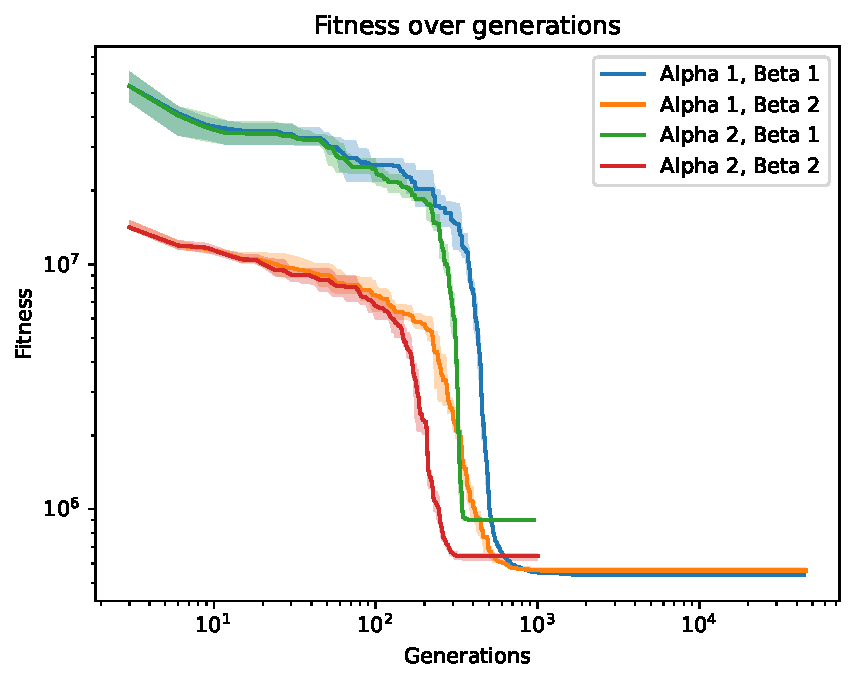
\includegraphics[width=\textwidth]{img/aco_random_ab.pdf}
        \caption{Randomly distributed data}
        \label{fig:aco_ab_random}
    \end{subfigure}
    \begin{subfigure}[b]{0.45\textwidth}
        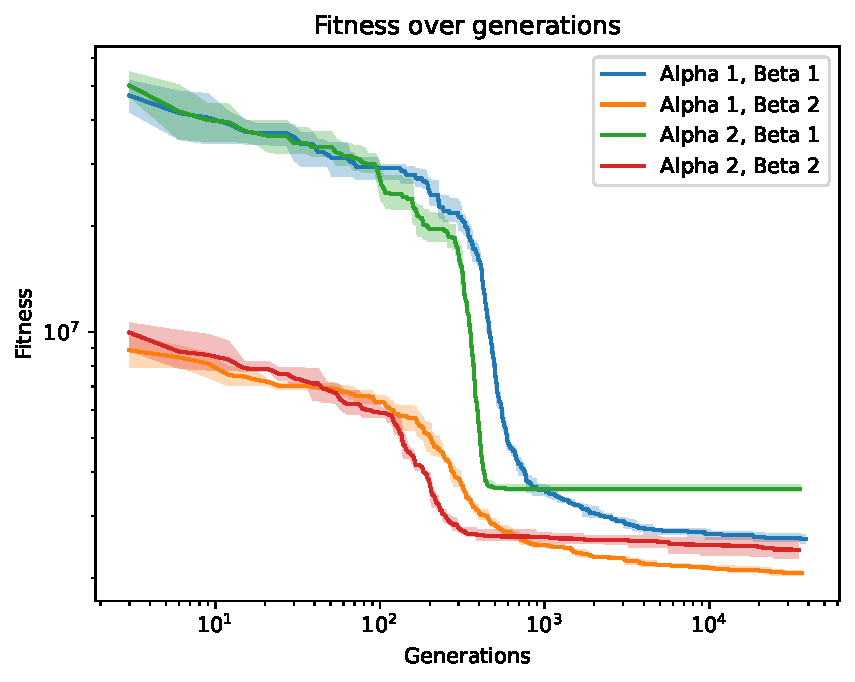
\includegraphics[width=\textwidth]{img/aco_commute_ab.pdf}
        \caption{Long distance commute data}
        \label{fig:aco_ab_commute}
    \end{subfigure}
    \caption{Ant Colony Optimization - Alpha and Beta setting}
    \label{fig:aco_alpha_beta}
\end{figure}

\begin{table}
    \centering
    \begin{tabular}{lc}
        $\alpha$ & 1 \\
        $\beta$ & 2 \\
        $\rho$ & 0.1 \\
        Number of ants & 20 \\
        Travel time weight in heuristic cost & 1 \\
        Time violation weight in heuristic cost & 2 \\
        Drop-off bonus coefficient & 10 \\
        Depot attractiveness coefficient & 0.1 \\
        Convergence factor to restart & 0.9999
    \end{tabular}
    \caption{Ant Colony Optimization - hyper-parameter settings}
    \label{tab:aco_hyperparams}
\end{table}

\section{Comparing different Ant Systems}

During development, we tried different versions of \textit{ACO} frameworks - \textit{Ant System (AS)}\cite{Dorigo2010}, $\mathcal{MM}$AS\cite{STUTZLE2000889} and \textit{HCF}\cite{HCFMMAS}. A comparison of these frameworks on datasets with $50$ customer requests can be seen in Figure~\ref{fig:aco_ant_systems}. All experiments ran for 20 minutes.

An important thing to note is that \textit{HCF} and \textit{$\mathcal{MM}$AS} use the same attractiveness function as described in \ref{sec:attractiveness}. However, for the \textit{AS}, we failed to find a single \textit{drop-off bonus coefficient} or different attractiveness function for which both datasets would converge to a reasonable solution. We therefore set the coefficient to $5$ for the commute dataset and $100$ for the random dataset. This is a major problem for the \textit{AS}, as it is less universal.

Based on the results, we decided to use only the \textit{HCF} in the final experiments, as it consistently outperformed the \textit{AS} and showed better characteristics during longer runs than the \textit{$\mathcal{MM}$AS}.

\begin{figure}
    \centering
    \begin{subfigure}[b]{0.45\textwidth}
        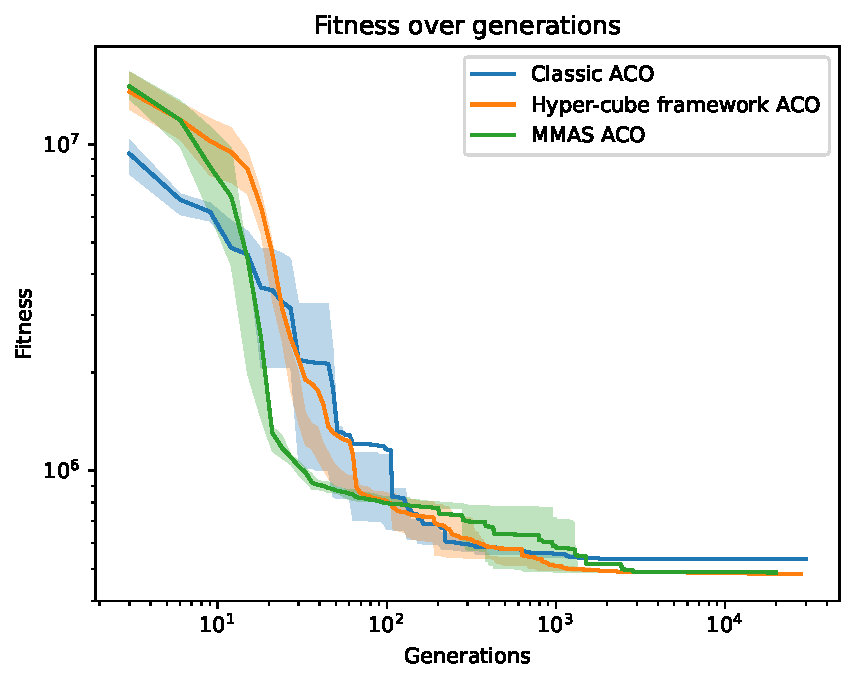
\includegraphics[width=\textwidth]{img/aco_compareas_random.pdf}
        \caption{Randomly distributed data}
        \label{fig:aco_as_random}
    \end{subfigure}
    \begin{subfigure}[b]{0.45\textwidth}
        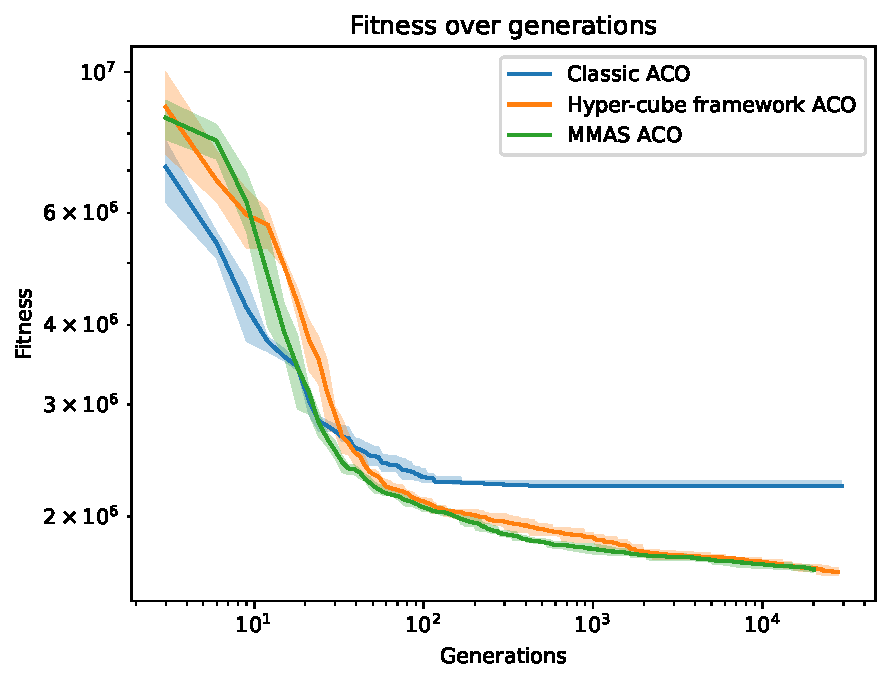
\includegraphics[width=\textwidth]{img/aco_compareas_commute.pdf}
        \caption{Long distance commute data}
        \label{fig:aco_as_commute}
    \end{subfigure}
    \caption{Ant Colony Optimization - Different Ant Systems}
    \label{fig:aco_ant_systems}
\end{figure}